\chapter{Problem set Solutions Fourier}
\begin{abox}
	Practise Set-1
\end{abox}
\begin{enumerate}[label=\color{ocre}\textbf{\arabic*.}]
	\item   The first few terms in the Laurent series for $\frac{1}{(z-1)(z-2)}$ in the region $1 \leq|z| \leq 2$ and around $z=1$ is
	{\exyear{NET/JRF(JUNE-2012)}}
	\begin{tasks}(1)
		\task[\textbf{A.}] $\frac{1}{2}\left[1+z+z^{2}+\ldots\right]\left[1+\frac{z}{2}+\frac{z^{2}}{4}+\frac{z^{3}}{8}+\ldots .\right]$
		\task[\textbf{B.}] $\frac{1}{1-z}-z-(1-z)^{2}+(1-z)^{3}+\ldots .$
		\task[\textbf{C.}] $\frac{1}{\mathrm{z}^{2}}\left[1+\frac{1}{\mathrm{z}}+\frac{1}{\mathrm{z}^{2}}+\ldots .\right]\left[1+\frac{2}{\mathrm{z}}+\frac{4}{\mathrm{z}^{2}}+\ldots . .\right]$
		\task[\textbf{D.}]  $2(z-1)+5(z-1)^{2}+7(z-1)^{3}+\ldots$
	\end{tasks}
	\begin{answer}
		\begin{align*}
		\frac{1}{(z-1)(z-2)}&=\frac{1}{z-2}-\frac{1}{z-1}=\frac{1}{1-z}+\frac{1}{(z-1)-1}\\&=\frac{1}{1-z}-(1+(1-z))^{-1}\\
		&=\frac{1}{1-z}-\left[1+(1-z)+\frac{(-1)(-2)}{2 !}(1-z)^{2}+\frac{(-1)(-2)(-3)}{3 !}(1-z)^{3} \ldots\right]\\
		&=\frac{1}{1-z}-\left[z+(1-z)^{2}-(1-z)^{3}+\ldots . .\right]
		\end{align*}
		So the correct answer is \textbf{Option (B)}
	\end{answer}
	\item Consider a sinusoidal waveform of amplitude $1 V$ and frequency $f_{0}$. Starting from an arbitrary initial time, the waveform is sampled at intervals of $\frac{1}{2 f_{0}}$. If the corresponding Fourier spectrum peaks at a frequency $\bar{f}$ and an amplitude $\bar{A}$, them
	{\exyear{NET/JRF(JUNE-2012)}}
	\begin{tasks}(2)
		\task[\textbf{A.}] $\bar{f}=2 f_{0}$ and $\bar{A}=1 V$
		\task[\textbf{B.}] $\bar{f}=2 f_{0}$ and $0 \leq \bar{A} \leq 1 V$
		\task[\textbf{C.}] $\bar{f}=0$ and $\bar{A}=1 V$
		\task[\textbf{D.}] $\bar{f}=\frac{f_{0}}{2}$ and $\bar{A}=\frac{1}{\sqrt{2}} V$
	\end{tasks}
	\begin{answer}$\left. \right. $
		\begin{figure}[H]
			\centering
			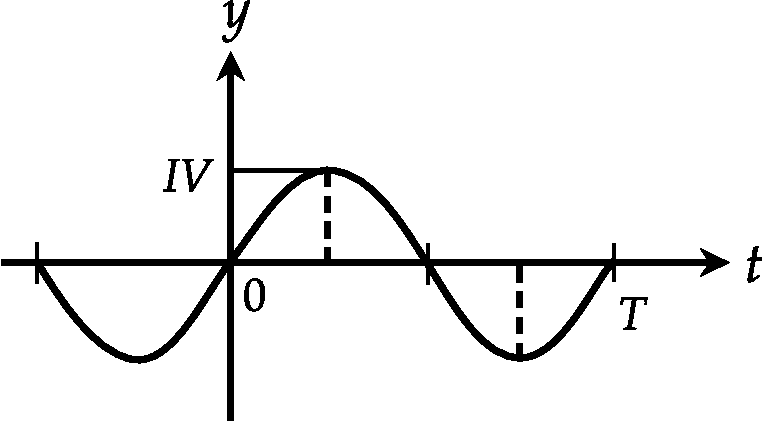
\includegraphics[height=4cm,width=8cm]{diagram-20211005(11)-crop}
		\end{figure}
		\begin{align*}
		y&=1 \sin \left(2 \pi f_{0} t\right)\\
		\text{The Fourier transform is:}\\
		F(y)&=\frac{1}{2}\left[\delta\left(f+f_{0}\right)\right]-\delta\left[f-f_{0}\right]\\
		\text{In Fourier domain }\bar{f}&=f_{0}, \bar{A}=\frac{1}{2}
		\end{align*}
		So the correct answer is \textbf{Option (B)}
	\end{answer}
	\item The Fourier transform of the derivative of the Dirac $\delta-$ function, namely $\delta^{\prime}(x)$, is proportional to
	{\exyear{NET/JRF(DEC-2013)}}
	\begin{tasks}(4)
		\task[\textbf{A.}] 0
		\task[\textbf{B.}] 1
		\task[\textbf{C.}] $\sin k$
		\task[\textbf{D.}] $i k$
	\end{tasks}
	\begin{answer}
		\begin{align*}
		\text{Fourier transform of }\delta^{\prime}(x)\\
		H(K)=\int_{-\infty}^{\infty} \delta^{\prime}(x) e^{i k x} d x&=i k e^{(k \cdot 0)}=i k
		\end{align*}
		So the correct answer is \textbf{Option (D)}
	\end{answer}
	\item The Laplace transform of $6 t^{3}+3 \sin 4 t$ is
	{\exyear{NET/JRF(JUNE-2015)}}
	\begin{tasks}(4)
		\task[\textbf{A.}] $\frac{36}{s^{4}}+\frac{12}{s^{2}+16}$
		\task[\textbf{B.}] $\frac{36}{s^{4}}+\frac{12}{s^{2}-16}$
		\task[\textbf{C.}] $\frac{18}{s^{4}}+\frac{12}{s^{2}-16}$
		\task[\textbf{D.}] $\frac{36}{s^{3}}+\frac{12}{s^{2}+16}$
	\end{tasks}
	\begin{answer}
		\begin{align*}
		L\left[6 t^{3}+3 \sin 4 t\right] &\quad \because L\left[t^{n}\right]=\frac{\sqrt{n+1}}{s^{n+1}}\\
		\because L[\sin a t]&=\frac{a}{\left(s^{2}+a^{2}\right)}\\
		L\left[6 t^{3}+3 \sin 4 t\right]&=\frac{6 \times \sqrt{4}}{s^{4}}+\frac{3 \times 4}{s^{2}+16}=\frac{36}{s^{4}}+\frac{12}{s^{2}+16}
		\end{align*}
		So the correct answer is \textbf{Option (A)}
	\end{answer}
	\item  The Fourier transform of $f(x)$ is $\tilde{f}(k)=\int_{-\infty}^{+\infty} d x e^{i k x} f(x)$.
	If $f(x)=\alpha \delta(x)+\beta \delta^{\prime}(x)+\gamma \delta^{\prime \prime}(x)$, where $\delta(x)$ is the Dirac delta-function (and prime denotes derivative), what is $\tilde{f}(k) ?$
	{\exyear{NET/JRF(DEC-2015)}}
	\begin{tasks}(2)
		\task[\textbf{A.}] $\alpha+i \beta k+i \gamma k^{2}$
		\task[\textbf{B.}] $\alpha+\beta k-\gamma k^{2}$
		\task[\textbf{C.}]  $\alpha-i \beta k-\gamma k^{2}$
		\task[\textbf{D.}] $i \alpha+\beta k-i \gamma k^{2}$
	\end{tasks}
	\begin{answer}
		\begin{align*}
		\tilde{f}(k)&=\int_{-\infty}^{\infty} d x e^{i k x}\left(\alpha \delta(x)+\beta \delta^{\prime}(x)+\gamma \delta^{\prime \prime}(x)\right)\\
		\int_{-\infty}^{\infty} \alpha \delta(x) e^{i k x} d x&=\alpha\\
		\int_{-\infty}^{\infty} \beta \delta^{\prime}(x) e^{i k x} d x&=\beta\left[\left.e^{i k x} \delta(x)\right|_{-\infty} ^{\infty}-\int_{-\infty}^{\infty} i k e^{i k x} \delta(x) d x\right]=-i \beta k\\
		\int_{-\infty}^{\infty} \gamma \delta^{\prime \prime}(x) e^{i k x} d x&=-\gamma k^{2}
		\end{align*}
		So the correct answer is \textbf{Option (C)}
	\end{answer}
	\item  What is the Fourier transform $\int d x e^{i l x} f(x)$ of
	$$
	f(x)=\delta(x)+\sum_{n=1}^{\infty} \frac{d^{n}}{d x^{n}} \delta(x)
	$$
	where $\delta(x)$ is the Dirac delta-function?
	{\exyear{NET/JRF(JUNE-2016)}}
	\begin{tasks}(4)
		\task[\textbf{A.}]  $\frac{1}{1-i k}$
		\task[\textbf{B.}] $\frac{1}{1+i k}$
		\task[\textbf{C.}] $\frac{1}{k+i}$
		\task[\textbf{D.}] $\frac{1}{k-i}$
	\end{tasks}
	\begin{answer}
		\begin{align*}
		f(x)&=\delta(x)+\sum_{n=1}^{\infty} \frac{d^{n}}{d x^{n}} \delta(x)\\&=\sum_{n=0}^{\infty} \frac{d^{n}}{d x^{n}} \delta(x)=\sum_{n=0}^{\infty} \delta^{(n)}(x)\\
		\because F[\delta(x)]&=1 \Rightarrow F\left[\delta^{(n)}(x)\right]\\&=(-i k)^{n} F[\delta(x)]=(-i k)^{n}\\
		\because f(x)&=\sum_{n=0}^{\infty} \delta^{(n)}(x)\\
		\Rightarrow F[f(x)]&=\sum_{n=0}^{\infty}(-i k)^{n}=1-i k+(i k)^{2}-(i k)^{3}+\ldots .\\&=\frac{1}{1-(-i k)}=\frac{1}{1+i k}
		\end{align*}
		So the correct answer is \textbf{Option (B)}
	\end{answer}
	\item The Laplace transform of
	$$
	f(t)=\left\{\begin{array}{cc}
	\frac{t}{T}, & 0<t<T \\
	1 & t>T
	\end{array}\right.
	$$
	is
	{\exyear{NET/JRF(DEC-2016)}}
	\begin{tasks}(4)
		\task[\textbf{A.}] $\frac{-\left(1-e^{-s T}\right)}{s^{2} T}$
		\task[\textbf{B.}] $\frac{\left(1-e^{-s T}\right)}{s^{2} T}$
		\task[\textbf{C.}] $\frac{\left(1+e^{-s T}\right)}{s^{2} T}$
		\task[\textbf{D.}] $\frac{\left(1-e^{s T}\right)}{s^{2} T}$
	\end{tasks}
	\begin{answer}
		\begin{align*}
		\intertext{we can write}
		f(t)&=\left[u_{0}(t)-u_{T}(t)\right] \frac{t}{T}+u_{T}(t)\\&=\left[1-u_{T}(t)\right] \frac{t}{T}+u_{T}(t)=\frac{t}{T}-u_{T}(t) \frac{t}{T}+u_{T}(t)
		\intertext{Hence the transform of $f(t)$ is}
		L\{f(t)\}&=L\left\{\frac{t}{T}\right\}-L\left\{u_{T}(t)\left[\frac{(t-T)+T}{T}\right]\right\}+L\left\{u_{T}(t)\right\}\\
		&=\frac{1}{s^{2} T}-\frac{e^{-s T}}{T}\left(\frac{1}{s^{2}}+\frac{T}{s}\right)+\frac{e^{-s T}}{s}=\frac{1-e^{-s T}}{s^{2} T}
		\end{align*}
		So the correct answer is \textbf{Option (B)}
	\end{answer}
	\item The Fourier transform $\int_{-\infty}^{\infty} d x f(x) e^{i k x}$ of the function $f(x)=\frac{1}{x^{2}+2}$ is
	{\exyear{NET/JRF(DEC-2016)}}
	\begin{tasks}(4)
		\task[\textbf{A.}] $\sqrt{2} \pi e^{-\sqrt{2}|| \mid}$
		\task[\textbf{B.}] $\sqrt{2} \pi e^{-\sqrt{2 k}}$
		\task[\textbf{C.}] $\frac{\pi}{\sqrt{2}} e^{-\sqrt{2 k}}$
		\task[\textbf{D.}] $\frac{\pi}{\sqrt{2}} e^{-\sqrt{2}|k|}$
	\end{tasks}
	\begin{answer}
		\begin{align*}
		\text{Fourier transform of }f(x)&=\frac{1}{x^{2}+a^{2}}, \\ a>0\text{ is }\int \frac{1}{x^{2}+a^{2}} e^{i k x} d x&=\frac{\pi}{a} e^{-a|k|}\\
		\text{Hence }\int \frac{1}{x^{2}+a^{2}} e^{i k x} d x&=\frac{\pi}{\sqrt{2}} e^{-\sqrt{2}|k|}
		\end{align*}
		So the correct answer is \textbf{Option (D)}
	\end{answer}
	\item Consider the differential equation $\frac{d y}{d t}+a y=e^{-b t}$ with the initial condition $y(0)=0$. Then the Laplace transform $Y(s)$ of the solution $y(t)$ is
	{\exyear{NET/JRF(DEC-2017)}}
	\begin{tasks}(4)
		\task[\textbf{A.}] $\frac{1}{(s+a)(s+b)}$
		\task[\textbf{B.}] $\frac{1}{b(s+a)}$
		\task[\textbf{C.}] $\frac{1}{a(s+b)}$
		\task[\textbf{D.}] $\frac{e^{-a}-e^{-b}}{b-a}$
	\end{tasks}
	\begin{answer}
		\begin{align*}
		\text{Given }\frac{d y}{d t}+a y&=e^{-b t}
		\intertext{Taking Laplace transform of both sides}
		\text{	We obtain}\\
		L\left\{\frac{d y}{d t}\right\}+a L\{y(t)\}&=L\left\{e^{-b t}\right\} \Rightarrow s Y(s)-y(0)+a Y(s)=\frac{1}{s+b}\\
		\text{Since, }	y(0)&=0,\text{ we obtain}\\
		(s+a) Y(s)&=\frac{1}{s+b} \Rightarrow Y(s)=\frac{1}{(s+a)(s+b)}
		\end{align*}
		So the correct answer is \textbf{Option (A)}
	\end{answer}
	\item  The Fourier transform $\int_{-\infty}^{\infty} d x f(x) e^{i k x}$ of the function $f(x)=e^{-|x|}$
	{\exyear{NET/JRF(JUNE-2018)}}
	\begin{tasks}(4)
		\task[\textbf{A.}] $-\frac{2}{1+k^{2}}$
		\task[\textbf{B.}] $-\frac{1}{2\left(1+k^{2}\right)}$
		\task[\textbf{C.}] $\frac{2}{1+k^{2}}$
		\task[\textbf{D.}] $\frac{2}{\left(2+k^{2}\right)}$
	\end{tasks}
	\begin{answer}
		\begin{align*}
		\int_{-\infty}^{+\infty} d x e^{-|x|} e^{i k x}&=\int_{-\infty}^{+\infty} d x e^{-|x|} \cos k x d x\text{ odd functions in }k x\text{ vanishes}\\
		\Rightarrow 2 \int_{0}^{\infty} e^{-x} \cos k x d x&=2 \frac{e^{-x}}{1+k^{2}}[-\cos k x+k \sin k x]_{0}^{\infty}\\
		\because \int e^{a x} \cos b x d x&=\frac{e^{a x}}{a^{2}+b^{2}}[a \cos b x+b \sin b x]\\
		\Rightarrow 2 \int_{0}^{\infty} e^{-x} \cos k x d x&=2 \frac{e^{0}}{1+k^{2}}=\frac{2}{1+k^{2}}
		\end{align*}
		So the correct answer is \textbf{Option (C)}
	\end{answer}
	\item The function $f(t)$ is a periodic function of period $2 \pi$. In the range $(-\pi, \pi)$, it equals $e^{-t}$. If $f(t)=\sum_{-\infty}^{\infty} c_{n} e^{\text {int }}$ denotes its Fourier series expansion, the sum $\sum_{-\infty}^{\infty}\left|c_{n}\right|^{2}$ is
	{\exyear{NET/JRF(DEC-2019)}}
	\begin{tasks}(4)
		\task[\textbf{A.}] 1
		\task[\textbf{B.}] $\frac{1}{2 \pi}$
		\task[\textbf{C.}] $\frac{1}{2 \pi} \cosh (2 \pi)$
		\task[\textbf{D.}]  $\frac{1}{2 \pi} \sinh (2 \pi)$
	\end{tasks}
	\begin{answer}
		\begin{align*}
		f(t)&=e^{-t} \quad-\pi<x<\pi\\
		f(t)&=\sum_{-\infty}^{\infty} c_{n} e^{\mathrm{int}}\\
		\sum_{-\infty}^{\infty}\left|c_{n}\right|^{2}&=\frac{1}{2 \pi} \int_{-\pi}^{\pi} e^{-2 t} d t=\left.\frac{1}{2 \pi} \cdot \frac{e^{-2 t}}{-2}\right|_{-\pi} ^{\pi}\\&=\frac{1}{2 \pi}\left[\frac{e^{-2 \pi}-e^{2 \pi}}{-2}\right]=\frac{1}{2 \pi} \sinh 2 \pi
		\end{align*}
		So the correct answer is \textbf{Option (D)}
	\end{answer}
\end{enumerate}
\colorlet{ocre1}{ocre!70!}
\colorlet{ocrel}{ocre!30!}
\setlength\arrayrulewidth{1pt}
\begin{table}[H]
	\centering
	\arrayrulecolor{ocre}
	\begin{tabular}{|p{1.5cm}|p{1.5cm}||p{1.5cm}|p{1.5cm}|}
		\hline
		\multicolumn{4}{|c|}{\textbf{Answer key}}\\\hline\hline
		\rowcolor{ocrel}Q.No.&Answer&Q.No.&Answer\\\hline
		1&\textbf{B} &2&\textbf{B}\\\hline 
		3&\textbf{D} &4&\textbf{A} \\\hline
		5&\textbf{C} &6&\textbf{B} \\\hline
		7&\textbf{B}&8&\textbf{D}\\\hline
		9&\textbf{A}&10&\textbf{C}\\\hline
		11&\textbf{D} &&\textbf{}\\\hline
		
	\end{tabular}
\end{table}

\newpage
\begin{abox}
	Practise Set-2
\end{abox}
\begin{enumerate}[label=\color{ocre}\textbf{\arabic*.}]
	\item If $f(x)=\left\{\begin{array}{ll}0 & \text { for } x<3, \\ x-3 & \text { for } x \geq 3\end{array}\right.$ then the Laplace transform of $f(x)$ is
	{\exyear{GATE 2010}}
	\begin{tasks}(4)
		\task[\textbf{A.}] $s^{-2} e^{3 s}$
		\task[\textbf{B.}] $s^{2} e^{3 s}$
		\task[\textbf{C.}] $s^{-2}$
		\task[\textbf{D.}] $s^{-2} e^{-3 s}$
	\end{tasks}
	\begin{answer}
		\begin{align*}
		L\{f(x)\}&=\int_{0}^{\infty} e^{-s x} f(x) d x\\&=\int_{0}^{3} e^{-s x} f(x) d x+\int_{3}^{\infty} e^{-s x} f(x) d x\\&=\int_{3}^{\infty}(x-3) e^{-s x} d x\\
		L\{f(x)\}&=\left.(x-3) \frac{e^{-s x}}{-s}\right|_{3} ^{\infty}-\int_{3}^{\infty} 1 \cdot\left(\frac{e^{-s x}}{-s}\right) d x\\&=0+\frac{1}{s} \int_{3}^{\infty} e^{-s x} d x\\&=\frac{1}{s}\left[\frac{e^{-s x}}{-s}\right]_{3}^{\infty}=s^{-2} e^{-3 s}
		\end{align*}
		So the correct answer is \textbf{Option (D)}
	\end{answer}
	\item The coefficient of $e^{i k x}$ in the Fourier expansion of $u(x)=A \sin ^{2}(\alpha x)$ for $k=-2 \alpha$ is
	{\exyear{GATE 2017}}
	\begin{tasks}(4)
		\task[\textbf{A.}] $\frac{A}{4}$
		\task[\textbf{B.}] $\frac{-A}{4}$
		\task[\textbf{C.}] $\frac{A}{2}$
		\task[\textbf{D.}] $\frac{-A}{2}$
	\end{tasks}
	\begin{answer}
		\begin{align*}
		\text{	Since, }\sin (\alpha x)&=\frac{e^{i \alpha x}-e^{-i \alpha x}}{2 i} \Rightarrow \sin ^{2}(\alpha x)\\&=\frac{e^{i 2 \alpha x}-2+e^{-2 i \alpha x}}{(-4)}\\
		\text{Since, }2 \alpha&=-k,\text{ hence }\sin ^{2}(\alpha x)\\&=\frac{e^{-i k x}-2+e^{i k x}}{(-4)}\\
		\text{Hence, }c_{k}&=\frac{A}{2 \pi} \int_{-\pi}^{\pi} \sin ^{2}(\alpha x) d x\\&=-\frac{A}{8 \pi}\left[\int_{-\pi}^{\pi} e^{-i k x} e^{-i k x} d x-2 \int_{-\pi}^{\pi} e^{-i k x} d x+\int_{-\pi}^{\pi} e^{-i k x} e^{i k x} d x\right]\\
		&=-\frac{A}{8 \pi}\left[\int_{-\pi}^{\pi} e^{-2 i k x} d x-2 \int_{-\pi}^{\pi} e^{-i k x} d x+\int_{-\pi}^{\pi} d x\right]
		\intertext{The first two integrals are zero and the third integral has the value $2 \pi$.
			Thus,}
		c_{k}&=-\frac{A}{8 \pi}(2 \pi)=-\frac{A}{4}
		\end{align*}
		So the correct answer is \textbf{Option (B)}
	\end{answer}
	\item Given the fundamental constants $\hbar$ (Planck's constant), $G$ (universal gravitation constant) and $c$ (speed of light), which of the following has dimension of length?
	{\exyear{JEST 2014}}
	\begin{tasks}(2)
		\task[\textbf{A.}]$\sqrt{\frac{\hbar G}{c^{3}}}$
		\task[\textbf{B.}] $\sqrt{\frac{\hbar G}{c^{5}}}$
		\task[\textbf{C.}]$\frac{\hbar G}{c^{3}}$
		\task[\textbf{D.}] $\sqrt{\frac{\hbar c}{8 \pi G}}$
	\end{tasks}
	\begin{answer}
		\begin{align*}
		\left[\frac{\left[M L^{2} T^{-1}\right]\left[M^{-1} L^{3} T^{-2}\right]}{L^{3} T^{-3}}\right]^{\frac{1}{2}}&=\left[L^{2}\right]^{\frac{1}{2}}=L\\
		\hbar=\left[M L^{2} T^{-1}\right], G=\frac{g r^{2}}{m}&=\left[M^{-1} L^{3} T^{-2}\right]
		\end{align*}
		So the correct answer is \textbf{Option (A)}
	\end{answer}
	\item The Fourier transform of the function $\frac{1}{x^{4}+3 x^{2}+2}$ up to proportionality constant is
	{\exyear{JEST 2017}}
	\begin{tasks}(2)
		\task[\textbf{A.}]$\sqrt{2} \exp \left(-k^{2}\right)-\exp \left(-2 k^{2}\right)$
		\task[\textbf{B.}]$\sqrt{2} \exp (-|k|)-\exp (-\sqrt{2}|k|)$
		\task[\textbf{C.}]$\sqrt{2} \exp (-\sqrt{|k|})-\exp (-\sqrt{2|k|})$
		\task[\textbf{D.}]  $\sqrt{2} \exp \left(-\sqrt{2} k^{2}\right)-\exp \left(-2 k^{2}\right)$
	\end{tasks}
	\begin{answer}
		\begin{align*}
		f(x)&=\frac{1}{\left(x^{4}+3 x^{2}+2\right)}=\frac{1}{\left(x^{2}+1\right)}-\frac{1}{\left[x^{2}+(\sqrt{2})^{2}\right]}
		\intertext{Now, Fourier transform of $f(x)$ is,}
		F(p)&=A \int_{-\infty}^{\infty} f(x) e^{-1 k x} d x\\
		&=A \int_{-\infty}^{\infty}\left[\frac{1}{\left(x^{2}+1\right)}-\frac{1}{x^{2}+(\sqrt{2})^{2}}\right] e^{-i k x} d x=A\left[\int_{-\infty}^{\infty} \frac{1}{\left(x^{2}+1\right)} \times e^{-i k x} d x-\int_{-\infty}^{\infty} \frac{e^{-i k x}}{x^{2}+(\sqrt{2})^{2}} d x\right]\\
		\because &\int_{-\infty}^{\infty} \frac{1}{\left(x^{2}+a^{2}\right)} e^{-i k x} d x=\sqrt{\frac{\pi}{2}} \frac{e^{-a|k|}}{a}\\
		F(k)&=A\left[\sqrt{\frac{\pi}{2}} \frac{e^{-|k|}}{1}-\sqrt{\frac{\pi}{2}} \frac{e^{-\sqrt{2} \mid k}}{\sqrt{2}}\right]=\frac{A \sqrt{\pi}}{2}[\sqrt{2} \exp (-|k|)-\exp (-\sqrt{2}|k|)]\\
		\end{align*}
		So the correct answer is \textbf{Option (B)}
	\end{answer}
	\item The function $f(x)=\cosh x$ which exists in the range $-\pi \leq x \leq \pi$ is periodically repeated between $x=(2 m-1) \pi$ and $(2 m+1) \pi$, where $m=-\infty$ to $\infty$. Using Fourier series, indicate the correct relation at $x=0$
	{\exyear{JEST 2017}}
	\begin{tasks}(2)
		\task[\textbf{A.}] $\sum_{n=-\infty}^{\infty} \frac{(-1)^{n}}{1-n^{2}}=\frac{1}{2}\left(\frac{\pi}{\cosh \pi}-1\right)$
		\task[\textbf{B.}]$\sum_{n=-\infty}^{\infty} \frac{(-1)^{n}}{1-n^{2}}=2 \frac{\pi}{\cosh \pi}$
		\task[\textbf{C.}]$\sum_{n=-\infty}^{\infty} \frac{(-1)^{-n}}{1+n^{2}}=2 \frac{\pi}{\sinh \pi}$
		\task[\textbf{D.}] $\sum_{n=1}^{\infty} \frac{(-1)^{n}}{1+n^{2}}=\frac{1}{2}\left(\frac{\pi}{\sinh \pi}-1\right)$
	\end{tasks}
	\begin{answer}
		\begin{align*}
		f(x)&=\cosh x, \quad-\pi \leq x \leq \pi\\
		\text{Here, }a_{0}&=\frac{1}{2 \pi} \int_{-\pi}^{\pi} \cosh x d x=\frac{1}{2 \pi}[\sinh x]_{-\pi}^{\pi}=\frac{\sinh \pi}{\pi}\\
		b_{n}&=0,\text{ due to even function}\\
		\text{	and }a_{n}&=\frac{1}{2 \pi} \int_{-\pi}^{\pi}\left(e^{x}+e^{-x}\right) \cos n x d x\qquad
		\left[\because \cosh x=\frac{1}{2}\left(e^{x}+e^{-x}\right)\right]\\
		a_{n}&=\frac{1}{2 \pi}\left[\frac{e^{x}}{\left(1+n^{2}\right)}(\cos n x+n \sin n x)+\frac{e^{-x}}{1+n^{2}}(-\cos n x+n \sin n x)\right]_{-\pi}^{\pi}\\
		&=\frac{1}{2 \pi}\left[\frac{e^{\pi}(-1)^{n}}{\left(1+n^{2}\right)}-\frac{e^{-\pi}(-1)^{n}}{\left(1+n^{2}\right)}-\frac{e^{-\pi}(-1)^{n}}{\left(1+n^{2}\right)}+\frac{e^{\pi}(-1)^{n}}{\left(1+n^{2}\right)}\right]\\&=\frac{2(-1)^{n} \cdot 2 \sinh \pi}{2 \pi\left(1+n^{2}\right)}=\frac{2(-1)^{n} \sinh \pi}{\pi\left(1+n^{2}\right)}\\
		\text{	Hence, }f(x)&=a_{0}+\sum_{n=1}^{\infty}\left(a_{n} \cos n x+b_{n} \sin n x\right) \Rightarrow \cosh x=\frac{\sinh \pi}{\pi}+\sum_{n=1}^{\infty} \frac{2(-1)^{n} \sinh \pi}{\pi\left(1+n^{2}\right)} \cos n x\\
		\text{At }x&=0,\\
		\sum_{n=1}^{\infty} \frac{2(-1)^{n} \sinh \pi}{\pi\left(1+n^{2}\right)}&=\left(1-\frac{\sinh \pi}{\pi}\right) \Rightarrow \sum_{n=1}^{\infty} \frac{(-1)^{n}}{\left(1+n^{2}\right)}=\frac{1}{2}\left[\frac{\pi}{\sinh \pi}-1\right]
		\end{align*}
		So the correct answer is \textbf{Option (D)}
	\end{answer}
	\item The Laplace transform of $\frac{(\sin (a t)-a t \cos (a t))}{\left(2 a^{3}\right)}$ is
	{\exyear{JEST 2018}}
	\begin{tasks}(2)
		\task[\textbf{A.}]$\frac{2 a s}{\left(s^{2}+a^{2}\right)^{2}}$
		\task[\textbf{B.}]$\frac{s^{2}-a^{2}}{\left(s^{2}+a^{2}\right)^{2}}$
		\task[\textbf{C.}]$\frac{1}{(s+a)^{2}}$
		\task[\textbf{D.}] $\frac{1}{\left(s^{2}+a^{2}\right)^{2}}$
	\end{tasks}
	\begin{answer}
		\begin{align*}
		L\left\{\frac{\sin a t-a t \cos a t}{2 a^{3}}\right\}=\frac{1}{\left(s^{2}+a^{2}\right)^{2}}
		\end{align*}
		So the correct answer is \textbf{Option (D)}
	\end{answer}
\end{enumerate}
\colorlet{ocre1}{ocre!70!}
\colorlet{ocrel}{ocre!30!}
\setlength\arrayrulewidth{1pt}
\begin{table}[H]
	\centering
	\arrayrulecolor{ocre}
	\begin{tabular}{|p{1.5cm}|p{1.5cm}||p{1.5cm}|p{1.5cm}|}
		\hline
		\multicolumn{4}{|c|}{\textbf{Answer key}}\\\hline\hline
		\rowcolor{ocrel}Q.No.&Answer&Q.No.&Answer\\\hline
		1&\textbf{D} &2&\textbf{B}\\\hline 
		3&\textbf{A} &4&\textbf{B} \\\hline
		5&\textbf{D} &6&\textbf{D} \\\hline
		
	\end{tabular}
\end{table}